\documentclass[12pt]{article}

\usepackage[margin=1in]{geometry}
\usepackage{setspace}
\usepackage{graphicx}
\usepackage{fancyhdr}
\usepackage{array}
\usepackage{titlesec}
\usepackage{lastpage}
\usepackage{biblatex}
\addbibresource{references.bib}
\usepackage{tikz}
\usepackage{float}
\setstretch{1.5}
\usepackage[table]{xcolor}
\usepackage{float}
\usepackage{caption}
\usepackage{tikz}
\usetikzlibrary{positioning}
%------------------ HEADER / FOOTER ------------------%
\pagestyle{fancy}
\fancyhf{}

% Header image (replace with actual filename)
\rhead{
\includegraphics[height=0.8cm]{header_logo.png}}
\lfoot{Robotics -- Spring 2026}

% \lfoot{Group Project Report}
\rfoot{Page \thepage \;of \pageref{LastPage}}

\renewcommand{\headrulewidth}{0.4pt}
\renewcommand{\footrulewidth}{0.4pt}

%------------------ SECTION STYLE ------------------%
\titleformat{\section}{\large\bfseries}{\thesection.}{1em}{}

\begin{document}

%------------------ TITLE PAGE ------------------%
\begin{titlepage}
\centering

\vspace*{1cm}

%------------------ TITLE ------------------%
{\Large \textbf{AI Trash Sorting Robot\\(Trashboat)}}

{\normalsize by} \\[0.5cm]

%------------------ TABLE ------------------%
\renewcommand{\arraystretch}{1.5}
\begin{tabular}{|c|}
\hline
\centering \textbf{Student Name} \tabularnewline
\hline
Owen Barnes\\ \hline
Felistus Karanja\\ \hline
Ryan Domathoti\\ \hline
Daniel Anoruo\\ \hline
Frankie Horter\\ \hline
Myles Burrows\\ \hline
\end{tabular}

\vspace{0.75cm}

%------------------ REPORT INFO ------------------%
{\large \textbf{Group Project Report}} \\[0.25cm]

In partial fulfillment of the requirements for \\[0.5cm]

{\large \textbf{COSC 465: Robotics}} \\
Spring-2026

\vfill

%------------------ SUBMITTED TO (RIGHT ALIGNED) ------------------%
\begin{flushright}
Submitted to \\
Anik Mallik, PhD \\
Assistant Professor \\
Department of Computer and Information Sciences \\
Towson University \\
Towson, MD
\end{flushright}

%------------------ DATE ------------------%
\centering
Date of submission: 05/12/2026
\end{titlepage}


%------------------ MAIN CONTENT ------------------%

\section*{Introduction}

For this project we created an AI-powered trash-sorting robot. The robot that takes in top-down images of our waste plate and sends it through a Convolution Neural Network. The network determines if the waste on the tray is one of three things: Trash, Compost, or Recycle. After determining what the object is, the plate holding the object will rotate to face the respective bin and drop the object into it.

The purpose of our robot is to completely automate the process of sorting between different types of waste. The problem with normal trash cans is that many times humans are lazy and careless and do not put in the mental effort to put their waste into the correct bin. This doesn't affect our individual lives but it harms our efforts to re-purpose recyclable and compost-able which which in turn harms our planet. Our robot removes the variable of carelessness from the equation as all three types of waste are dropped onto the same plate and our automated process does the rest of the work.

This project used topics covered by the lecture notes on Computer Vision, AI \& Deep Learning, Dynamics \& Actuators, and finally Transformation, Rotation, Joints, and Degrees of Freedom. All of these were extremely helpful when creating certain elements of the project.

\section*{Literature Review}
Currently in the field, there are several forms of this kind of project. We were originally inspired by the sorting cameras in our University Union. It was a system where you show your garbage to a camera, and it will tell you which bin you should place your garbage. This was designed by Intuitive AI's product, Oscar Sort\cite{sort_2014}.
We also took inspiration on the design of robot from the Bulgarian company, Ameru\cite{ameru_2025} with their product Smart Bin.
Both of these real-life products were major inspirations for the design of our robot, combining ideas of both products into one.

\section*{Design and Assembly Description}

\subsection{Mechanical Design \& Methods Used}

We adopted two main systems for the physical build: a Planetary Gear System and a Tilting Table System. 

\begin{itemize}
    \item \textbf{Planetary Gear System:} We chose this for the main drive because it handles high torque in a small space. By using multiple gears to share the load, the robot can move heavy trash without straining the motor. Our design features an integrated outer ring gear that includes dedicated mounting points for the tilting system motors.
\end{itemize}

\begin{figure}[H]
    \centering
    
\includegraphics[width=0.6\linewidth]{source//Phase 1 Images/Screenshot 2026-05-12 113837.png}
    \caption{Planetary Gear Assembly with Integrated Tilting Motor Mounts}
    \label{fig:planetary_gear}
\end{figure}

\begin{itemize}
    \item \textbf{Tilting Table System:} This was designed for the actual sorting action. It uses a pivot point to quickly dump items into specified bins. By mounting the tilting motors directly onto the planetary ring, we reduced the overall footprint and improved mechanical stability.
\end{itemize}
\subsection{Custom Fabrication and Component Modeling}

To ensure seamless mechanical integration, a rigorous custom fabrication process was followed. This involved:

\begin{itemize}
    \item \textbf{Motor Measurement and Modeling:} All actuators, including the primary Nema 17 driver and Servo tilting motors, were  measured using precision calipers to establish exact dimensions for shaft diameter, mounting hole patterns and overall housing volume. These measurements were then used to create accurate 3D CAD models of each motor.
    \begin{figure}[H]
    \centering
    
\includegraphics[width=0.4\linewidth]{source//Phase 1 Images/Capture 1.PNG}
    
\includegraphics[width=0.4\linewidth]{source//Phase 1 Images/Capture 17.PNG}
    \caption{Nema 17 and Servo motor Cad Models}
    \label{fig:planetary_gear}
\end{figure}
    \item \textbf{Integrated Chassis Design:} Using these models, the planetary gear housing was custom-designed to serve as both a gearbox and a structural chassis. The motor mounts were modeled directly into the ring gear to ensure zero-tolerance fitment and eliminate mechanical play during high-torque operations.
    \item \textbf{Tolerance Management:} We accounted for 3D printing and measurement discrepancies by padding all measurement by 0.02mm This ensured that the custom-fabricated gears meshed smoothly with the motors without the need for extensive post-processing.
\end{itemize}

\subsubsection{Assembled Design}
With the assembled design, we have different containers for Trash, Recycling \& Compost as well as a live feed of what the camera sees.
\begin{figure}[h]
    \centering
    
\includegraphics[width=1\linewidth]{LaTeX Report/IMG_6718.jpg}
    \caption{The assembled, finalized design of the Trashboat}
    \label{fig:fullDesign}
\end{figure}

\newpage
\subsubsection{Component Wiring}
Here we have the Arduino, Raspberry Pi, and Nemo motor on the inside of the container, as well as wire managment.
\begin{figure}[h]
    \centering
    
\includegraphics[width=0.5\linewidth]{LaTeX Report/IMG_6721.jpg}
    \caption{The inner-workings/wiring of Trashboat}
    \label{fig:wiring}
\end{figure}

\subsection{System Workflow}

\begin{itemize}
    \item \textbf{Assembly:} The planetary gearbox acts as the primary structural base. The tilting motors are secured into the built-in housings on the ring gear, which then drive the sorting plate.
    \item \textbf{Operation:} The planetary gears provide the rotational positioning, while the integrated motors trigger the tilting motion once the robot reaches the target bin.
\end{itemize}


\section*{AI Waste Classification Pipeline}
We compared the performance of 3 neural networks on their ability to classify trash, recycle, and compost items across 12k+ images. These models included a Custom Convolutional Neural Network (CNN) engineered from scratch, ResNet18, and YOLOv8.

\begin{figure}[H]
\centering

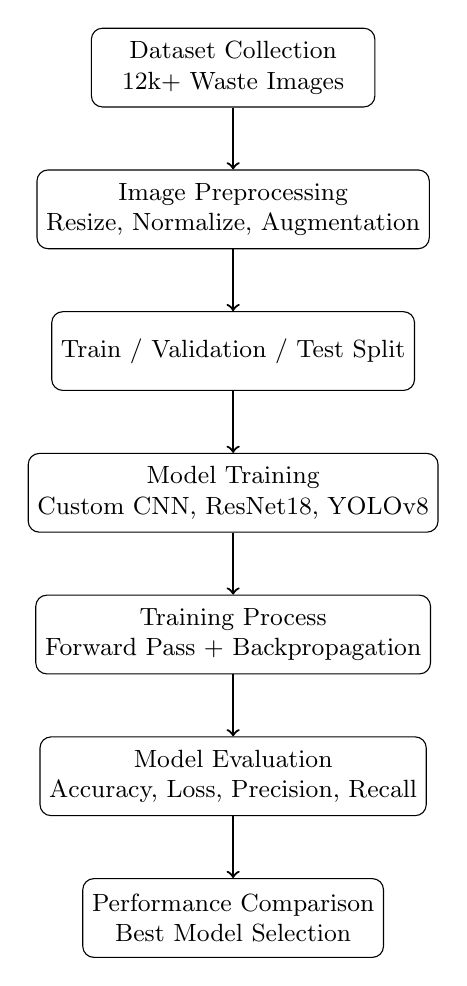
\begin{tikzpicture}[
    node distance=1.8cm,
    every node/.style={font=\small},
    process/.style={
        rectangle,
        draw,
        rounded corners,
        minimum width=3.6cm,
        minimum height=1cm,
        align=center
    },
    arrow/.style={->, thick}
]

% Nodes
\node (dataset) [process] {Dataset Collection\\12k+ Waste Images};

\node (preprocess) [process, below of=dataset] 
{Image Preprocessing\\Resize, Normalize, Augmentation};

\node (split) [process, below of=preprocess] 
{Train / Validation / Test Split};

\node (models) [process, below of=split] 
{Model Training\\Custom CNN, ResNet18, YOLOv8};

\node (train) [process, below of=models] 
{Training Process\\Forward Pass + Backpropagation};

\node (evaluate) [process, below of=train] 
{Model Evaluation\\Accuracy, Loss, Precision, Recall};

\node (compare) [process, below of=evaluate] 
{Performance Comparison\\Best Model Selection};

% Arrows
\draw [arrow] (dataset) -- (preprocess);
\draw [arrow] (preprocess) -- (split);
\draw [arrow] (split) -- (models);
\draw [arrow] (models) -- (train);
\draw [arrow] (train) -- (evaluate);
\draw [arrow] (evaluate) -- (compare);

\end{tikzpicture}

\caption{Deep learning training pipeline used for waste classification across trash, recycle, and compost datasets.}
\label{fig:ai_pipeline}
\end{figure}

Our custom CNN processes images through convolutional layers that quickly learn important features such as edges, shapes, and textures. Following the convolutional Layers, we use ReLU activation functions, which help the network learn more complex patterns in the images. And finally, the Max pooling layers reduce the image size while keeping the most important information for classification.

\begin{figure}[H]
    \centering
    
\includegraphics[width=0.95\linewidth]{source//Phase 1 Images/cnn.png}
    \caption{Custom CNN Architecture for Waste Classification}
    \label{fig:cnn_architecture}
\end{figure}


ResNet18 is a special kind of CNN, that also processes images through deep convolutional layers to learn important features such as edges, shapes, textures, and object patterns. Following the convolutional layers, the model uses Batch Normalization and ReLU activation functions to improve training stability and help the network learn more complex image representations. ResNet18 also uses residual shortcut connections, which allow the model to pass information between layers more efficiently while reducing performance degradation in deeper networks.

\begin{figure}[H]
    \centering
    
\includegraphics[width=0.95\linewidth]{source//Phase 1 Images/resnet18.png}
    \caption{ResNet18 Architecture for Waste Classification}
    \label{fig:cnn_architecture}
\end{figure}

YOLOv8 is an enhanced CNN architecture that is utilized for image classification and real-time object detection. Following the convolutional layers, the model uses Batch Normalization and SiLU activation functions, which help the network learn more complex patterns while improving training performance. And finally, the detection head predicts the class and location of objects while keeping the most important information needed for accurate classification and detection.

\begin{figure}[H]
    \centering
    
\includegraphics[width=0.8\linewidth]{source//Phase 1 Images/yolov8.png}
    \caption{Yolov8 Architecture for Waste Classification}
    \label{fig:cnn_architecture}
\end{figure} 

\section{Computer Vision Implementation}
Using Raspberry Pi as the processing unit, we were able to both run our AI models in real time through our pipeline system. Utilizing OpenCV, we created a loop that is triggered via motion detection, constantly comparing the previous frame
 to the current frame to detect movement. This process was implemented for when an item is dropped into the plate of our robot. 
 
 \begin{table}[H]
\centering
\caption{Motion Detection State System}
\label{tab:motion_states}

\begin{tabular}{|l|p{10cm}|}
\hline
\rowcolor[HTML]{0B5D7A}
\textcolor{white}{\textbf{State}} & 
\textcolor{white}{\textbf{Description}} \\ \hline

\textbf{LIVE} & 
Camera feed is active, waiting for motion. \\ \hline

\textbf{WAIT} & 
Short delay to stabilize object before capture. \\ \hline

\textbf{CAPTURED} & 
Image is frozen and processed. \\ \hline

\textbf{DISPLAY} & 
Result is shown for a fixed duration. \\ \hline

\end{tabular}
\end{table}
 
 The system is split into 4 states: Live, Wait, Captured, and Display, where large amounts of detected movement transition the system from the Live state into the Wait and Captured stages before finally displaying the classification results. This process is also live-streamed from the camera feed into Flask for real-time monitoring through a web interface. The label predicted is then sent to the Arduino to move the object into the correct bin.

\section*{Evaluation Metrics}
\begin{table}[H]
\caption{Evaluation Metrics Used for Model Performance}
\centering
\begin{tabular}{|p{3cm}|p{9cm}|}
\hline
\textbf{Metric} & \textbf{Description} \\ \hline

Accuracy &
Measures the overall percentage of correct predictions made by the model. \\ \hline

Precision &
Out of all predicted positives, how many were actually correct. \\ \hline

Recall &
Out of all actual positives, how many were correctly identified by the model. \\ \hline

F1-Score &
Represents the balance between precision and recall using their harmonic mean. \\ \hline

\end{tabular}
\label{tab:metrics}
\end{table}

After training, we conducted experiments over 10 iterations to evaluate which model performed best for real-time classification and detection. These repeated tests helped analyze the consistency, stability, and overall effectiveness of each model in live deployment scenarios.




\section*{Performance Results and Discussion}
In general, all models performed relatively well during on all 3 datasets (Training, Testing, and Validation datasets), the problems arose when we had to modify our model for real time classification/detection.

\subsection{Custom CNN Performance}
Our custom-built Convolutional Neural Network (CNN) performed well across the training, testing, and validation datasets. The model achieved an accuracy of approximately 98--99\% on the training dataset while averaging around 95\% on both the testing and validation datasets. Overall, the model demonstrated strong performance and consistency during classification tasks.


\begin{figure}[H]
\centering

\begin{minipage}{0.58\textwidth}
    \centering
    
\includegraphics[width=\linewidth]{source/Metrics/cnnperformance.png}
    \caption{Custom CNN Accuracy}
    \label{fig:yoloaccuracy}
\end{minipage}
\hfill
\begin{minipage}{0.35\textwidth}
    \centering

    \textbf{CNN Evaluation Metrics}

    \vspace{0.3cm}

    \begin{tabular}{|c|c|}
    \hline
    \textbf{Metric} & \textbf{Score (\%)} \\ \hline

    Accuracy & 95.2 \\ \hline
    Precision & 94.8 \\ \hline
    Recall & 94.3 \\ \hline
    F1-Score & 94.5 \\ \hline

    \end{tabular}

\end{minipage}

\end{figure}

Despite these metrics, when we deployed our model for real-time detection, it performed poorly in correctly classifying objects in live environments. To further evaluate performance, we conducted 10 real-time classification iterations using different waste items. Out of the 10 iterations, only 4 classifications were correct.

\vspace{0.2cm}

\small

\begin{center}
\begin{tabular}{|c|c|c|}
\hline
\textbf{Iteration} & \textbf{Predicted Output} & \textbf{Actual Output} \\ \hline

\rowcolor{green!20}
1 & Trash & Trash \\ \hline

2 & Recycle & Compost \\ \hline

\rowcolor{green!20}
3 & Recycle & Recycle \\ \hline

4 & Compost & Trash \\ \hline

\rowcolor{green!20}
5 & Compost & Compost \\ \hline

6 & Trash & Recycle \\ \hline

7 & Compost & Trash \\ \hline

8 & Recycle & Trash \\ \hline

\rowcolor{green!20}
9 & Trash & Trash \\ \hline

10 & Compost & Recycle \\ \hline

\end{tabular}
\end{center}

\normalsize
\subsection{ResNet18 Performance}
Similar to our custom-built neural network, the ResNet18 model performed exceptionally well across all datasets. The model achieved an accuracy of nearly 100\% on the training dataset while maintaining approximately 97--98\% accuracy on both the testing and validation datasets. Overall, the model demonstrated strong generalization and high classification performance.
\begin{figure}[H]
\centering

\begin{minipage}{0.52\textwidth}
    \centering
    
\includegraphics[width=\linewidth]{source/Metrics/resnet18performance.png}
    \caption{ResNet18 Performance}
    \label{fig:resnet18performance}
\end{minipage}
\hfill
\begin{minipage}{0.43\textwidth}
    \centering

    \textbf{ResNet18 Classification Metrics by Class}

    \vspace{0.2cm}

    \small

    \begin{tabular}{|c|c|c|c|}
    \hline
    \textbf{Class} & \textbf{Precision} & \textbf{Recall} & \textbf{F1} \\ \hline

    Trash & 0.880 & 0.920 & 0.900 \\ \hline
    Compost & 0.965 & 0.966 & 0.965 \\ \hline
    Recycle & 0.935 & 0.924 & 0.930 \\ \hline
    Accuracy & 0.951 & 0.951 & 0.951 \\ \hline

    \end{tabular}

    \normalsize

\end{minipage}
\end{figure}

Despite these metrics, when we deployed the ResNet18 model for real-time detection, the model still struggled with consistent object classification in live environments. Out of the 10 iterations, only 5 classifications were correct.

\vspace{0.2cm}

\small

\begin{center}
\begin{tabular}{|c|c|c|}
\hline
\textbf{Iteration} & \textbf{Predicted Output} & \textbf{Actual Output} \\ \hline

\rowcolor{green!20}
1 & Recycle & Recycle \\ \hline

\rowcolor{green!20}
2 & Recycle & Recycle \\ \hline

\rowcolor{green!20}
3 & Recycle & Recycle \\ \hline

4 & Compost & Trash \\ \hline

5 & Trash & Compost \\ \hline

\rowcolor{green!20}
6 & Trash & Trash \\ \hline

7 & Recycle & Compost \\ \hline

\rowcolor{green!20}
8 & Trash & Trash \\ \hline

9 & Compost & Recycle \\ \hline

10 & Trash & Compost \\ \hline

\end{tabular}
\end{center}

\normalsize

\subsection{YoloV8 Performance}
\begin{samepage}

This model performed well overall, with the training pipeline recording a testing dataset accuracy of approximately 98\%. Compared to the previous models, it achieved the highest testing accuracy, demonstrating stronger overall classification performance and generalization capabilities.

\vspace{0.2cm}

\begin{center}

\begin{minipage}[c]{0.47\textwidth}
    \centering
    
\includegraphics[width=0.95\linewidth]{source/Metrics/yolov8accuracy.png}
    
    \vspace{0.1cm}
    \small Figure: YOLOv8 Testing Accuracy
\end{minipage}
\hspace{0.005\textwidth}
\begin{minipage}[c]{0.47\textwidth}
    \centering

    \small
    \textbf{YOLOv8 Classification Metrics}

    \vspace{0.15cm}

    \begin{tabular}{|c|c|c|c|}
    \hline
    \textbf{Class} & \textbf{Precision} & \textbf{Recall} & \textbf{F1} \\ \hline
    Compost & 0.97 & 0.97 & 0.97 \\ \hline
    Recycle & 0.98 & 0.98 & 0.98 \\ \hline
    Trash & 0.98 & 0.98 & 0.98 \\ \hline
    Accuracy & 0.98 & 0.98 & 0.98 \\ \hline
    \end{tabular}

\end{minipage}

\end{center}

\end{samepage}

When deploying our model for real-time waste detection and classification, it achieved higher performance in comparison to the previous models. Out of the 10 iterations, the model correctly classified 8 of the waste items. Further testing showed that the model performed exceptionally well when classifying compost and recycle materials in comparison to trash items.

\vspace{0.2cm}

\small

\begin{center}
\begin{tabular}{|c|c|c|}
\hline
\textbf{Iteration} & \textbf{Predicted Output} & \textbf{Actual Output} \\ \hline

\rowcolor{green!20}
1 & Recycle & Recycle \\ \hline

\rowcolor{green!20}
2 & Recycle & Recycle \\ \hline

\rowcolor{green!20}
3 & Recycle & Recycle \\ \hline

\rowcolor{green!20}
4 & Compost & Compost \\ \hline

\rowcolor{green!20}
5 & Compost & Compost \\ \hline

\rowcolor{green!20}
6 & Compost & Compost \\ \hline

7 & Compost & Trash \\ \hline

\rowcolor{green!20}
8 & Trash & Trash \\ \hline

\rowcolor{green!20}
9 & Trash & Trash \\ \hline

10 & Recycle & Trash \\ \hline

\end{tabular}
\end{center}

\normalsize

\section*{Challenges}
\indent The system faced both hardware and software challenges. Upon first gaining access to hardware, physical limitations proved to be a significant challenge. The original servos moved 180 degrees although our logic utilized a 360 degree model which we had adapted to. We faced power limitations when wiring the servos to the Arduino as each servo was not receiving enough power. External sources through outlets were utilized.
\newline
There were also time constraints that led to some patch-job fixes with certain hardware elements. For example, there was not enough time to remake the outer gear from the planetary gear system, so we modified it to account for the shift in the tilting table system.
\newline
\indent Configuring a learning model to detect trash was difficult as we had researched many alternatives that would give us accurate readings. some models incorrectly identified objects with a trash or recycle bias. Adjusting parameter weights and increasing the amount of model data helped us to give more accurate readings.
\newline
\indent A significant software challenge was enabling communication between the Raspberry Pi and the Arduino. Both the Raspberry Pi and Arduino have USB-A and USB-C ports so using those main USB channels, direct communication between the microcomputer and micro controller were possible through serial port 9600. 
\newline

\section*{Future Work}
\indent Although the AI Trash Detecting Robot provided strong results, much could be improved on. 
\newline
\indent Firstly the servo assembly could be cleaned up a little more. The servos are held in place by friction which over time will eventually fail. Having a dedicated housing in plastic composite or stamped metal would help with the integrity of the robot. 
\newline
\indent Having the model self train itself would only prove to be beneficial to the environment around it. Implementing a user input "Check or X" option to tell whether the robot was right or not would help increase the accuracy of the model.
\newline
\indent The application of this would work in a low density area like a bedroom, living room, or office cubicle. For larger applications like cafeterias and public parks, the turntable design would need to act quicker and more efficiently from object detection to sorting the object. 

\section*{Conclusion}
\indent In conclusion, the AI Trash Sorting Robot demonstrates how robotics and deep learning can be combined to automate waste separation efficiently. By integrating computer vision, neural network classification, mechanical actuation, and digital logic, the system successfully identifies waste items. These items are then distributed into their respective locations(Trash, Recycle, Compost). Our testing showed that machine learning models can provide accurate predictions when deployed on hardware such as the Raspberry Pi. Although challenges such as real-time performance and hardware limitations were encountered, they provided valuable opportunities for improvement and learning. Overall, this project shows strong potential for future waste management systems that can reduce human error and support environmental sustainability.

\section*{References}
\nocite{*}
\printbibliography[heading=none]

\newpage
\section*{Appendices }
\subsection{Training Hyperparameters}

The following hyperparameters were used during the training experiments for the deep learning models.

\vspace{0.2cm}

\begin{table}[H]
\centering
\caption{Training Hyperparameters}
\begin{tabular}{|c|c|}
\hline
\textbf{Hyperparameter} & \textbf{Value} \\ \hline

Learning Rate & $1 \times 10^{-4}$ \\ \hline

Epochs & 200 \\ \hline

Optimizer & Adam Optimizer \\ \hline

Loss Function & CrossEntropy Loss \\ \hline

\end{tabular}
\label{tab:hyperparameters}
\end{table}
\vspace{1cm}

\section{Robot Communication Pipeline}

The following diagram demonstrates how the Raspberry Pi processes images using the YOLOv8 classifier and sends the predicted waste category to the Arduino micro controller, which then controls the movement of the robot.

\vspace{0.4cm}

\begin{figure}[H]
\centering

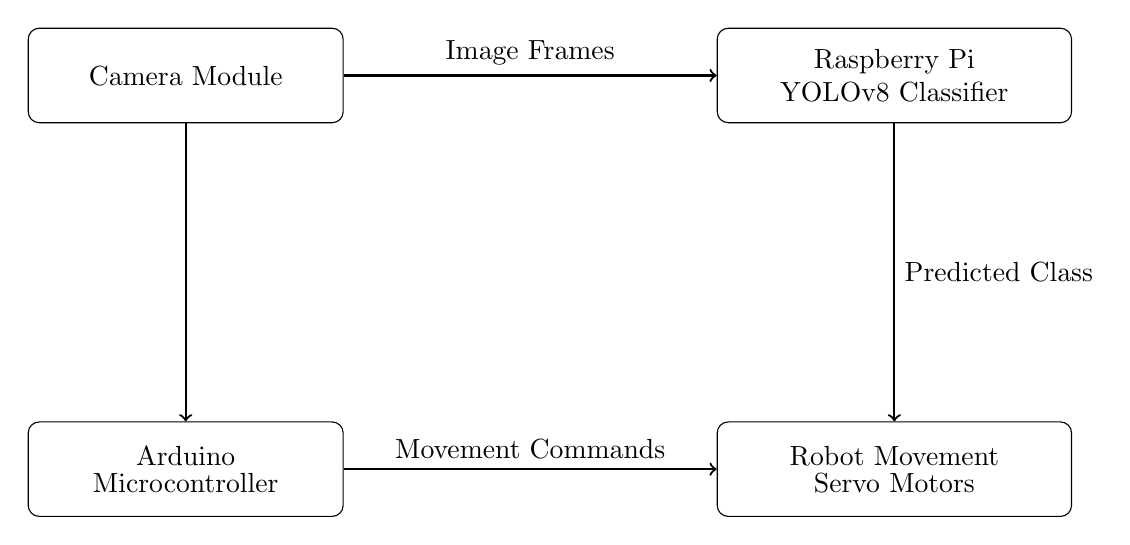
\begin{tikzpicture}[every node/.style={align=center}]

% Top Row
\node[
draw,
rounded corners,
minimum width=4cm,
minimum height=1.2cm
] (camera) at (0,0)
{\shortstack{Camera Module}};

\node[
draw,
rounded corners,
minimum width=4.5cm,
minimum height=1.2cm
] (rpi) at (9,0)
{\shortstack{Raspberry Pi \\ YOLOv8 Classifier}};

% Bottom Row
\node[
draw,
rounded corners,
minimum width=4cm,
minimum height=1.2cm
] (arduino) at (0,-5)
{\shortstack{Arduino \\ Microcontroller}};

\node[
draw,
rounded corners,
minimum width=4.5cm,
minimum height=1.2cm
] (robot) at (9,-5)
{\shortstack{Robot Movement \\ Servo Motors}};

% Arrows
\draw[->, thick] (camera) -- node[above]
{\hspace{0.3cm}Image Frames\hspace{0.3cm}} (rpi);

\draw[->, thick] (rpi) -- node[right, align=center]
{\shortstack{Predicted Class}} (robot);

\draw[->, thick] (camera) -- (arduino);

\draw[->, thick] (arduino) -- node[above]
{\hspace{0.3cm}Movement Commands\hspace{0.3cm}} (robot);

\end{tikzpicture}

\caption{YOLOv8 Waste Classification Communication Pipeline}
\label{fig:robotpipeline}

\end{figure}


\end{document}
